% Informe final - IA Fundamentals (UTEC). Máximo 4 páginas.
% Compilar desde informe/: tectonic main.tex  (o pdflatex + bibtex). Las figuras de resultados se leen de ../figuras/.
% En Overleaf: subir el repositorio completo y compilar informe/main.tex.
\documentclass[conference,a4paper]{IEEEtran}

% Funciona con XeTeX/LuaTeX (Tectonic) y con pdfLaTeX (Overleaf por defecto).
\usepackage{iftex}
\ifTUTeX
  \usepackage{fontspec}
  % TeX Gyre Termes: equivalente libre de Times, la fuente de IEEEtran (cargada por archivo)
  \setmainfont{texgyretermes}[Extension=.otf, UprightFont=*-regular, BoldFont=*-bold,
    ItalicFont=*-italic, BoldItalicFont=*-bolditalic]
  \setmonofont{texgyrecursor}[Extension=.otf, UprightFont=*-regular, BoldFont=*-bold,
    ItalicFont=*-italic, BoldItalicFont=*-bolditalic]
\else
  \usepackage[utf8]{inputenc}
  \usepackage[T1]{fontenc}
\fi
\usepackage[spanish,es-noshorthands,es-tabla,es-nodecimaldot]{babel}
\usepackage{amsmath}
\usepackage{booktabs}
\usepackage{tabularx}
\usepackage{array}
\usepackage{graphicx}
\usepackage{xcolor}
\usepackage{url}
\usepackage{cite}

\graphicspath{{figuras/}{../figuras/}}% pipeline en informe/figuras; resultados en ../figuras (figuras_informe.py)
\newcommand{\pendiente}[1]{\textcolor{red}{[#1]}}
\newcolumntype{L}{>{\raggedright\arraybackslash}X}
% Separación más compacta alrededor de figuras y tablas (límite de 4 páginas)
\setlength{\textfloatsep}{8pt plus 2pt minus 2pt}
\setlength{\dbltextfloatsep}{8pt plus 2pt minus 2pt}
\setlength{\floatsep}{6pt plus 2pt minus 2pt}
\setlength{\dblfloatsep}{6pt plus 2pt minus 2pt}

\begin{document}

\title{Detección de clientes con fraude en la banca digital peruana mediante ensembles balanceados}

\author{\IEEEauthorblockN{Junior Godofredo Baldeon Blas, Adnan Ahmed Choudary Ahmed, Eduardo Sebastián Lévano Cavero,\\
Michelle Yunorvi Luna Alama, Diego Alonso Ortiz Vera}
\IEEEauthorblockA{Maestría en Ciencia de Datos e IA, Universidad de Ingeniería y Tecnología (UTEC), Lima, Perú\\
Curso: AI Fundamentals. Docente: Vicente Machaca Arceda}}

\maketitle

% =======================================================================================
\begin{abstract}
Este trabajo compara cuatro modelos base (regresión logística, árbol de decisión, KNN y
XGBoost) para ordenar a clientes de banca digital por riesgo de fraude, con el conjunto «Data
fraude bancario en Perú» (5\,960 clientes, 3,51\,\% con fraude confirmado). Cada modelo se
integra en un mismo ensemble de 30 submuestras balanceadas, y datos, preprocesamiento,
particiones (validación cruzada estratificada $5\times5$) y métricas son idénticos para todos. La regresión logística obtuvo la mayor PR-AUC ($0{,}168 \pm 0{,}040$, frente a
$0{,}035$ del azar) y, revisando el 5\,\% de clientes con mayor riesgo, encontró el 26,6\,\%
de los fraudes. Las pruebas estadísticas pareadas muestran que el árbol de decisión es
significativamente peor y que la ventaja de la regresión logística sobre XGBoost y KNN es
consistente, pero pequeña.
\end{abstract}

% =======================================================================================
\section{Introducción}

La detección de fraude en la banca digital requiere identificar casos sospechosos sin
saturar de alertas a los clientes legítimos. El aprendizaje automático permite combinar el
perfil, el comportamiento y la seguridad de los usuarios para priorizar qué casos revisar, pero
la tarea se dificulta porque los clientes con fraude son una fracción pequeña.

Este trabajo usa el conjunto «Data fraude bancario en Perú»~\cite{kaggle}, con 5\,960 clientes
y 27 variables; 209 clientes (3,51\,\%) tienen fraude confirmado. Cada fila es un cliente y no
una transacción. Con este desbalance, un clasificador que declare a todos los clientes sin
fraude alcanza una exactitud de 96,49\,\% sin detectar un solo caso. Por eso el problema se
plantea como \emph{ordenar} a los clientes por riesgo y medir cuántos fraudes quedan entre los
primeros que se revisarían.

Se comparan cuatro modelos base (regresión logística, árbol de decisión, $k$ vecinos más
cercanos o KNN, y XGBoost) dentro de un mismo ensemble de 30 submuestras balanceadas; todo lo
demás se mantiene fijo para atribuir las diferencias al modelo base.

La regresión logística obtuvo la mayor PR-AUC media (0,168 frente a 0,035 del azar) y, al
revisar el 5\,\% de clientes con mayor puntaje, encontró el 26,6\,\% de los fraudes con una
precisión de 18,5\,\%; XGBoost y KNN quedaron cerca y el árbol de decisión, claramente por
debajo. El código y los resultados están disponibles en
\url{https://github.com/Diegortizv/deteccion-fraude-banca-peru}.

% =======================================================================================
\section{Trabajos relacionados}

Los trabajos revisados difieren sobre todo en cómo tratan el desbalance de clases y cómo
evalúan. Tres implementaciones públicas usan las 284\,807 transacciones con tarjeta de la
Université Libre de Bruxelles (0,172\,\% de fraudes).
modi02~\cite{modi02} aplica sobremuestreo tipo SMOTE solo al entrenamiento y compara
regresión logística, Random Forest y Gradient Boosting, con F1 de 0,72, 0,86 y 0,86; pero sus
cifras son autorreportadas y el código usa datos sintéticos si falta el archivo original. anahitapouladi~\cite{anahitapouladi}
separa entrenamiento, validación y prueba (60/20/20) y pondera las clases; en validación,
Random Forest obtiene una precisión promedio de 0,874 frente a 0,787 de la regresión logística,
y en prueba, con el umbral elegido en validación, detecta 68 de 95 fraudes (recall de
71,6\,\%) con 2 falsas alarmas. El propio trabajo reconoce que una partición aleatoria no mide
la respuesta ante fraudes futuros. NusraatMili~\cite{nusraatmili} compara Naive Bayes, árbol
de decisión, Random Forest, KNN ($k=15$) y regresión logística; Random Forest obtiene el mejor
resultado (F1 de 0,92 y ROC-AUC de 0,993), mientras que KNN logra un ROC-AUC de 0,964 pero un
F1 de solo 0,08, lo que muestra que una métrica con umbral fijo y una de ordenamiento pueden
llevar a conclusiones opuestas.

Entre los artículos, Mienye y Swart~\cite{mienye2024} generan transacciones fraudulentas
sintéticas con una red generativa adversaria (GAN) y usan redes recurrentes como
discriminador; su modelo GAN-GRU alcanza una sensibilidad de 0,992 y una especificidad de 1,000
en el conjunto europeo. Rugeles Diaz
et al.~\cite{rugeles2025} analizan 221\,292 registros de tarjetas de una pasarela de pagos
latinoamericana (2022), segmentan los comercios y eligen modelos según su tamaño, con Random
Forest o árbol de decisión (Gini) como respaldo; con ellos se habría evitado entre 48\,\% y
85\,\% de los fraudes, aunque advierten que los modelos deben actualizarse porque los
defraudadores cambian de técnica. Estos trabajos analizan transacciones de otros conjuntos, así que
sus cifras no son comparables con las nuestras, y \cite{modi02,anahitapouladi} evalúan en una
sola partición. Este trabajo aborda el fraude a nivel de cliente, fija todo salvo el modelo
base y compara en 25 particiones con pruebas estadísticas pareadas.

% =======================================================================================
\section{Propuesta}\label{sec:propuesta}

\begin{figure*}[t]
\centering
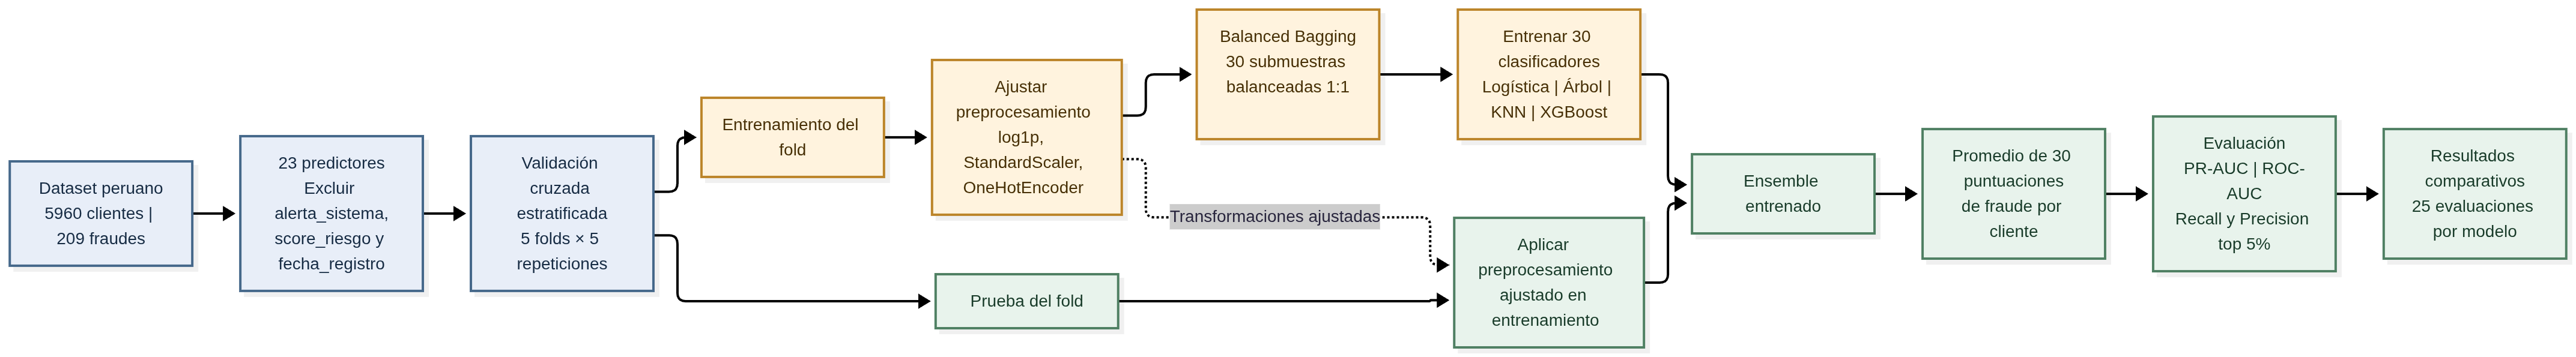
\includegraphics[width=\textwidth]{pipeline.png}
\caption{Pipeline propuesto. Solo cambia el modelo base entre experimentos.}
\label{fig:pipeline}
\end{figure*}

Se propone un enfoque de aprendizaje supervisado: como el conjunto incluye una etiqueta
confirmada (\texttt{fraude\_confirmado}, 1 = fraude), un modelo puede aprender de clientes etiquetados
a estimar el riesgo de otros~\cite{leborgne2022}. La \textbf{entrada} son
23 variables de cada cliente: perfil (edad, ingreso, antigüedad, departamento, banco),
comportamiento (app, tipo de operación, montos, frecuencia), canales (cajeros, agencias, POS) y
diez indicadores de seguridad (p.\,ej., ubicación inusual, dispositivo nuevo, intentos de
contacto sospechoso). La
\textbf{salida} es un puntaje de riesgo entre 0 y 1, con el que se ordena a los clientes de
mayor a menor riesgo: una lista de prioridad para analistas que solo pueden revisar una parte
(Fig.~\ref{fig:pipeline}).

\textbf{Columnas excluidas.} \texttt{alerta\_sistema} y \texttt{score\_riesgo} son salidas de
otro sistema antifraude: la primera, sola, alcanza un ROC-AUC de 0,815, y la segunda se explica
casi por completo con los diez indicadores de seguridad ($R^2 = 0{,}938$). Usarlas mediría al
sistema anterior y no a nuestro modelo (fuga de información o \emph{leakage}).
\texttt{fecha\_registro} es artificial: los 5\,960 registros comparten la misma hora del día,
lo que sugiere, como otros indicios, que los datos son sintéticos.

\textbf{Preprocesamiento.} El ingreso y los montos son muy asimétricos (monto de operación:
mediana S/~193, máximo S/~11\,091), por eso se les aplica $\log(1+x)$ antes de estandarizar
(Tabla~\ref{tab:condiciones}); todo se ajusta solo con el entrenamiento, para no usar
información de prueba~\cite{leborgne2022}.

\textbf{Ensemble balanceado.} Se entrenan 30 modelos, cada uno con todos los fraudes del
entrenamiento y la misma cantidad de clientes sin fraude elegidos al azar, y el puntaje final
es el promedio de los 30 puntajes (EasyEnsemble~\cite{liu2009}). Cada submuestra
obliga al modelo a aprender la clase minoritaria; usar 30 recupera la información que una sola
descartaría, y promediar reduce la varianza~\cite{breiman1996}.
Se prefirió a SMOTE~\cite{chawla2002} porque la mayoría de indicadores de seguridad son binarios
o conteos, y la interpolación crearía valores imposibles (p.\,ej., dispositivo nuevo = 0,37).
El submuestreo infla los puntajes~\cite{dalpozzolo2015}, así que no deben leerse como
probabilidades reales; no se calibran porque las métricas usadas solo dependen del orden.

% =======================================================================================
\section{Experimentos}\label{sec:experimentos}

Con todo lo demás fijo (Tabla~\ref{tab:condiciones}), los experimentos responden: \emph{¿qué
familia de modelo base (Tabla~\ref{tab:modelos}) ordena mejor a los clientes por riesgo de
fraude?}

\begin{table}[t]
\caption{Condiciones experimentales, idénticas en E0--E4}
\label{tab:condiciones}
\centering
\footnotesize
\renewcommand{\arraystretch}{1.1}
\begin{tabularx}{\columnwidth}{@{}>{\bfseries}p{1.55cm} L@{}}
\toprule
Datos & 5\,960 clientes (209 fraudes). Objetivo: \texttt{fraude\_confirmado}. 23 predictores: 19 numéricos, 4 categóricos. \\
Partición & Validación cruzada estratificada, 5 folds $\times$ 5 repeticiones (semilla 42): 25 pares. Entrenamiento: 4\,768 clientes (167--168 fraudes); prueba: 1\,192 (41--42). \\
Validación & No hay: los hiperparámetros se fijan de antemano (Tabla~\ref{tab:modelos}) y el fold de prueba no interviene en ninguna decisión. \\
Preproce\-samiento & $\log(1+x)$ y estandarización a ingreso y 2 montos; estandarización a las otras 16 numéricas; \emph{one-hot} a las 4 categóricas (categorías no vistas se ignoran): 46 variables. Parámetros calculados solo con el fold de entrenamiento. \\
Entrena\-miento & 30 submuestras 1:1 del fold de entrenamiento (todos sus fraudes y el mismo número de no fraudes, sin reemplazo: 334--336 filas); un modelo base por submuestra. E0 es un solo modelo, sin submuestras. \\
Predicción & Promedio de los 30 puntajes de cada cliente de prueba. \\\\
Evaluación & 4 métricas por fold de prueba: 25 valores por modelo, resumidos con media $\pm$ desviación estándar (DE). \\
Compara\-ción & Friedman, Nemenyi y Wilcoxon-Holm sobre PR-AUC, $\alpha = 0{,}05$~\cite{demsar2006}. \\
Reprodu\-cibilidad & Semilla 42; scikit-learn 1.6.1~\cite{pedregosa2011}, imbalanced-learn 0.13.0~\cite{lemaitre2017} y XGBoost 2.1.4~\cite{chen2016}; huella SHA-256 del archivo de datos verificada. \\
\bottomrule
\end{tabularx}
\end{table}

\begin{table}[t]
\caption{Experimentos (E1 es el caso base): solo cambia el modelo base}
\label{tab:modelos}
\centering
\footnotesize
\begin{tabularx}{\columnwidth}{@{}l p{3.05cm} L@{}}
\toprule
Exp. & Modelo (familia) & Hiperparámetros fijos \\
\midrule
E0 & Dummy (azar) & al azar, sin ensemble (piso de referencia) \\
E1 & Reg. logística (lineal) & $C=1$, L2, máx.\ 2000 iteraciones \\
E2 & Árbol de decisión (reglas) & completo, sin podar \\
E3 & KNN (distancias) & $k=15$ vecinos \\
E4 & XGBoost (\emph{boosting})~\cite{chen2016} & 300 árboles, profundidad 4, tasa de aprendizaje 0,05, submuestreo 0,8 de filas y columnas \\
\bottomrule
\end{tabularx}
\end{table}

\textbf{Métricas.} En cada fold de prueba se ordena a los 1\,192 clientes por su puntaje, de
mayor a menor. Sea el \emph{top 5\,\%} el grupo de los 60 primeros. El \emph{recall top 5\,\%}
es la fracción de los fraudes del fold que quedan en ese grupo, y la \emph{precisión top 5\,\%}
es la fracción de esos 60 clientes que tienen fraude; ambas simulan la capacidad de revisión de
un equipo de analistas sin fijar un umbral~\cite{leborgne2022}. La \emph{PR-AUC}
(\emph{average precision}) recorre el orden completo y promedia la precisión acumulada en cada
posición donde aparece un fraude:
\begin{equation}
\text{PR-AUC} = \frac{1}{F}\sum_{j=1}^{F} \frac{j}{r_j},
\end{equation}
donde $F$ es el número de fraudes del fold y $r_j$ es la posición del $j$-ésimo fraude en el
orden. Vale 1 si todos los fraudes quedan primero y, al azar, se acerca a la prevalencia (0,035).
El \emph{ROC-AUC} es la probabilidad de que un cliente con fraude reciba mayor puntaje que uno sin
fraude; vale 0,5 al azar. La PR-AUC es la métrica principal porque se concentra en la parte alta
del orden, que es la que se revisa, mientras que el ROC-AUC puede ser alto solo por ordenar bien
a la gran mayoría sin fraude~\cite{saito2015}.

\textbf{Pruebas estadísticas.} Como los modelos se evalúan sobre los mismos 25 folds, se usan
pruebas pareadas no paramétricas~\cite{demsar2006}. \emph{Friedman}: en cada fold se ordenan
los cuatro modelos por PR-AUC (1 = mejor), se promedian esas posiciones (rango medio) y se
prueba si los rangos medios difieren más de lo esperable si los modelos fueran equivalentes.
\emph{Nemenyi}: si Friedman es significativa, dos modelos difieren cuando sus rangos medios se
separan más que la diferencia crítica
$CD = q_{0{,}05}\sqrt{k(k+1)/6N} = 2{,}569\sqrt{4\cdot5/(6\cdot25)} = 0{,}94$, con $k=4$
modelos y $N=25$ folds. \emph{Wilcoxon de rangos con signo}: compara E2, E3 y E4 con el caso
base E1 a partir de sus 25 diferencias de PR-AUC fold a fold. \emph{Holm}: ajusta esos tres
p-valores (el menor se multiplica por 3, el siguiente por 2 y el mayor por 1) para que la
probabilidad de declarar por error alguna diferencia siga siendo 5\,\%. Se reporta también la diferencia de medias (tamaño del efecto).

\textbf{Hipótesis.} En los datos, la señal se concentra en pocos indicadores: la tasa de fraude
es 12,7\,\% con ubicación inusual frente a 2,0\,\% sin ella, y 6,6\,\% con dispositivo nuevo
frente a 2,4\,\%, mientras que departamento, banco y app tienen tasas planas (1,8\,\% a
4,1\,\%) y aportan 19 de las 46 variables. Se espera que E0 dé una PR-AUC $\approx 0{,}035$
(control del cálculo); que E1 sea competitivo, porque esos efectos parecen sumarse; que el
ensemble reduzca la alta varianza del árbol y lo vuelva competitivo (E2)~\cite{breiman1996};
que KNN sea el más débil, porque las variables sin señal también entran en la distancia (E3); y
que XGBoost capte interacciones, pero pueda sobreajustar con submuestras de unas 335 filas (E4).

\textbf{Justificación.} Los modelos cubren cuatro formas de aprender (frontera lineal,
reglas, distancias y \emph{boosting}) y son los usados en los antecedentes: regresión
logística, árbol, KNN y ensembles de árboles en~\cite{modi02,anahitapouladi,nusraatmili}, y
árbol de decisión en~\cite{rugeles2025}; XGBoost~\cite{chen2016} representa el
\emph{gradient boosting} que compara~\cite{modi02}.

% =======================================================================================
\section{Resultados}\label{sec:resultados}

\begin{table*}[t]
\caption{Resultados: media $\pm$ DE en los 25 folds de prueba. Rango medio en PR-AUC entre E1 y E4 (1 = mejor). En negrita, el mejor valor}
\label{tab:resultados}
\centering
\footnotesize
\begin{tabular}{@{}llccccc@{}}
\toprule
Exp. & Modelo & PR-AUC & ROC-AUC & Recall top 5\,\% & Precisión top 5\,\% & Rango medio \\
\midrule
E0 & Dummy (azar) & $0{,}035 \pm 0{,}001$ & $0{,}496 \pm 0{,}012$ & $0{,}037 \pm 0{,}028$ & $0{,}026 \pm 0{,}019$ & -- \\
E1 & Regresión logística & $\mathbf{0{,}168 \pm 0{,}040}$ & $0{,}824 \pm 0{,}031$ & $\mathbf{0{,}266 \pm 0{,}048}$ & $\mathbf{0{,}185 \pm 0{,}033}$ & $\mathbf{1{,}60}$ \\
E2 & Árbol de decisión & $0{,}104 \pm 0{,}021$ & $0{,}791 \pm 0{,}027$ & $0{,}171 \pm 0{,}052$ & $0{,}119 \pm 0{,}036$ & $3{,}92$ \\
E3 & KNN & $0{,}147 \pm 0{,}025$ & $\mathbf{0{,}827 \pm 0{,}024}$ & $0{,}248 \pm 0{,}049$ & $0{,}173 \pm 0{,}034$ & $2{,}40$ \\
E4 & XGBoost & $0{,}151 \pm 0{,}031$ & $0{,}824 \pm 0{,}026$ & $0{,}251 \pm 0{,}066$ & $0{,}175 \pm 0{,}046$ & $2{,}08$ \\
\bottomrule
\end{tabular}
\end{table*}

\textbf{Controles.} La proporción de fraudes en los folds de prueba va de 3,44\,\% a 3,52\,\%,
y E0 obtiene una PR-AUC de 0,035 y un ROC-AUC de 0,496, los valores esperados del azar
(Tabla~\ref{tab:resultados}). Esto confirma que métricas y particiones se calculan bien.

\textbf{Comparación global.} Los cuatro modelos superan claramente al azar: su PR-AUC va de 3,0
veces la prevalencia (árbol) a 4,8 veces (regresión logística). En la
Fig.~\ref{fig:boxplot}, las cajas de E1, E3 y E4 se solapan, y la regresión logística es la de
mayor dispersión entre folds (PR-AUC de 0,100 a 0,253). La prueba de Friedman confirma que hay diferencias entre los cuatro modelos
($\chi^2 = 45{,}19$; $p = 8{,}4\times10^{-10}$). El ROC-AUC, en cambio, casi no los distingue (KNN tiene el mayor, 0,827), porque premia
ordenar bien a la mayoría sin fraude~\cite{saito2015}.

\begin{figure}[t]
\centering
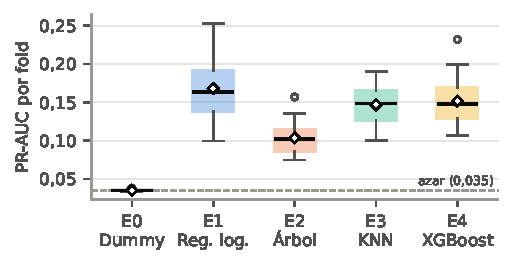
\includegraphics[width=\columnwidth]{boxplot_comparado.pdf}
\caption{PR-AUC en los 25 folds de prueba (rombo: media; línea punteada: prevalencia).}
\label{fig:boxplot}
\end{figure}

\begin{table}[t]
\caption{Comparación de E2--E4 con el caso base E1 (PR-AUC)}
\label{tab:pruebas}
\centering
\footnotesize
\setlength{\tabcolsep}{3.5pt}
\begin{tabular}{@{}lcccc@{}}
\toprule
 & Folds que & Diferencia & $p$ Wilcoxon & Dif.\ de rango \\
Modelo & gana E1 & de medias & (Holm) & (Nemenyi) \\
\midrule
E2 Árbol & 24 de 25 & $-0{,}064$ & $3{,}6\times10^{-7}$ & $2{,}32^{*}$ \\
E3 KNN & 20 de 25 & $-0{,}022$ & $1{,}1\times10^{-3}$ & $0{,}80$ \\
E4 XGBoost & 16 de 25 & $-0{,}017$ & $6{,}7\times10^{-3}$ & $0{,}48$ \\
\bottomrule
\multicolumn{5}{@{}l}{\scriptsize $^{*}$ Mayor que $CD = 0{,}94$: diferencia significativa según Nemenyi.}
\end{tabular}
\end{table}

\textbf{Comparación por pares.} Según Nemenyi (Tabla~\ref{tab:pruebas}), el árbol es significativamente peor que los otros tres (también frente a
XGBoost y KNN: diferencias de rango 1,84 y 1,52), pero E1, E3 y E4 no se separan entre sí;
Wilcoxon-Holm, en cambio, encuentra una PR-AUC menor que la de E1 en los tres. No se contradicen:
Nemenyi solo usa posiciones y compara los seis pares a la vez, por lo que es más exigente;
Wilcoxon usa el tamaño de cada diferencia en tres comparaciones. La regresión logística supera
de forma consistente a XGBoost y KNN, pero por poco (unos 0,02 de PR-AUC; frente a XGBoost gana
16 de 25 folds).

\textbf{Lectura operativa.} En el primer fold, la regresión logística colocó 14 de los 41
fraudes entre los 60 clientes con mayor puntaje, y solo 1 entre los 600 con menor puntaje. En
promedio (Fig.~\ref{fig:captura}), revisando el 5\,\% de clientes encuentra el 27\,\% de los
fraudes, unos 11 de 42, cuando al azar se encontrarían unos 2; revisando el 20\,\%, encuentra el
65\,\%, frente a 67\,\% de KNN, 63\,\% de XGBoost y 56\,\% del árbol. Las bandas de la Fig.~\ref{fig:captura}
muestran que la variación entre folds supera a las diferencias entre E1, E3 y E4: revisando el
5\,\%, E1 encuentra entre el 19\,\% y el 31\,\% de los fraudes según el fold, mientras que los
tres se separan en unos 2 puntos (y en 4 o menos desde el 20\,\%); por eso se comparan fold
a fold.

\begin{figure}[t]
\centering
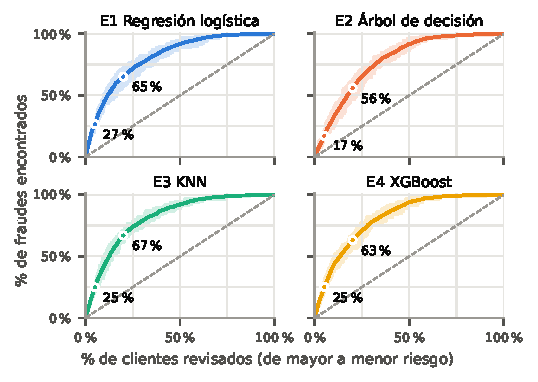
\includegraphics[width=\columnwidth]{captura_paneles.pdf}
\caption{Fraudes encontrados según los clientes revisados, de mayor a menor puntaje. Línea:
promedio de los 25 folds; banda: percentiles 10--90 entre folds; puntos: revisión del 5\,\% y
del 20\,\%. La diagonal es el azar.}
\label{fig:captura}
\end{figure}

\textbf{Contraste con las hipótesis.} \emph{E1 se cumple}: es la mejor opción, coherente
con una señal concentrada en pocos indicadores de efecto aditivo. \emph{E2 no se cumple}: el árbol es el peor en todas las métricas y su curva precisión-recall
es casi plana (en la repetición 1, precisión de 0,10--0,12 para recall de 0,05 a 0,60; la regresión logística, 0,14--0,27): separa a los clientes de bajo riesgo, pero no concentra
los fraudes arriba. La causa es que cada árbol completo termina en hojas puras y vota 0 o 1, así
que el promedio de 30 árboles solo toma unos 31 valores distintos y, en promedio, 27 clientes
empatan en el puesto 60.
\emph{E3 no se cumple}: KNN no es el más débil; queda a 0,005 de XGBoost en PR-AUC y muy por
encima del árbol. \emph{E4 se cumple en parte}: XGBoost queda segundo y tiene la mayor
variabilidad en el recall top 5\,\% (DE 0,066), pero sin comparar el error de entrenamiento y
de prueba no se puede atribuir a sobreajuste.

\textbf{Limitaciones.} Los datos probablemente son sintéticos y con más fraude que lo
habitual; los hiperparámetros son fijos; no se mide cuánto aporta el ensemble a cada modelo; las
métricas top 5\,\% del árbol dependen del desempate (orden de las filas), y como los folds
comparten clientes, los p-valores son aproximados.

% =======================================================================================
\section{Conclusiones}

Con el preprocesamiento, las 25 particiones y el ensemble fijos, la regresión logística fue el
modelo base que mejor priorizó a los clientes con fraude (PR-AUC de 0,168, unas 4,8 veces el
azar). Conviene ser precisos: frente a XGBoost y KNN la ventaja es de apenas 0,02 y Nemenyi no
los separa; el único resultado claramente peor fue el del árbol.

En la práctica, revisando el 5\,\% de clientes con mayor puntaje se encuentra uno de cada cuatro
fraudes, unas cinco veces más que al azar, pero casi tres de cada cuatro quedan fuera. Por eso
estos modelos sirven para ordenar el trabajo de los analistas, no para sustituir su criterio.

No todas las hipótesis se cumplieron. Esperábamos que el ensemble volviera competitivo al árbol,
y terminó último: sus votos 0 o 1 generan empates que restan finura al orden en las primeras
posiciones, una explicación coherente con los datos, pero no comprobada con un experimento. KNN
no fue el más débil y XGBoost quedó en un punto intermedio. Sí se cumplió que la regresión
logística fuera competitiva, lo que sugiere una señal concentrada en pocas variables de seguridad.

Estos resultados valen para este conjunto, probablemente sintético. Como continuación, proponemos
ajustar los hiperparámetros, medir el aporte del ensemble frente a cada modelo por separado,
cuantificar el efecto de las variables excluidas por fuga de información y validar el enfoque con
datos reales y una evaluación en el tiempo.

\bibliographystyle{IEEEtran}
\bibliography{referencias}

\end{document}
